
% Default to the notebook output style

    


% Inherit from the specified cell style.




    
\documentclass{article}

    
    
    \usepackage{graphicx} % Used to insert images
    \usepackage{adjustbox} % Used to constrain images to a maximum size 
    \usepackage{color} % Allow colors to be defined
    \usepackage{enumerate} % Needed for markdown enumerations to work
    \usepackage{geometry} % Used to adjust the document margins
    \usepackage{amsmath} % Equations
    \usepackage{amssymb} % Equations
    \usepackage{eurosym} % defines \euro
    \usepackage[mathletters]{ucs} % Extended unicode (utf-8) support
    \usepackage[utf8x]{inputenc} % Allow utf-8 characters in the tex document
    \usepackage{fancyvrb} % verbatim replacement that allows latex
    \usepackage{grffile} % extends the file name processing of package graphics 
                         % to support a larger range 
    % The hyperref package gives us a pdf with properly built
    % internal navigation ('pdf bookmarks' for the table of contents,
    % internal cross-reference links, web links for URLs, etc.)
    \usepackage{hyperref}
    \usepackage{longtable} % longtable support required by pandoc >1.10
    \usepackage{booktabs}  % table support for pandoc > 1.12.2

    \graphicspath{ {C:\Users\TrungDuy\Dropbox\MLproject} }

    
    
    \definecolor{orange}{cmyk}{0,0.4,0.8,0.2}
    \definecolor{darkorange}{rgb}{.71,0.21,0.01}
    \definecolor{darkgreen}{rgb}{.12,.54,.11}
    \definecolor{myteal}{rgb}{.26, .44, .56}
    \definecolor{gray}{gray}{0.45}
    \definecolor{lightgray}{gray}{.95}
    \definecolor{mediumgray}{gray}{.8}
    \definecolor{inputbackground}{rgb}{.95, .95, .85}
    \definecolor{outputbackground}{rgb}{.95, .95, .95}
    \definecolor{traceback}{rgb}{1, .95, .95}
    % ansi colors
    \definecolor{red}{rgb}{.6,0,0}
    \definecolor{green}{rgb}{0,.65,0}
    \definecolor{brown}{rgb}{0.6,0.6,0}
    \definecolor{blue}{rgb}{0,.145,.698}
    \definecolor{purple}{rgb}{.698,.145,.698}
    \definecolor{cyan}{rgb}{0,.698,.698}
    \definecolor{lightgray}{gray}{0.5}
    
    % bright ansi colors
    \definecolor{darkgray}{gray}{0.25}
    \definecolor{lightred}{rgb}{1.0,0.39,0.28}
    \definecolor{lightgreen}{rgb}{0.48,0.99,0.0}
    \definecolor{lightblue}{rgb}{0.53,0.81,0.92}
    \definecolor{lightpurple}{rgb}{0.87,0.63,0.87}
    \definecolor{lightcyan}{rgb}{0.5,1.0,0.83}
    
    % commands and environments needed by pandoc snippets
    % extracted from the output of `pandoc -s`
    \providecommand{\tightlist}{%
      \setlength{\itemsep}{0pt}\setlength{\parskip}{0pt}}
    \DefineVerbatimEnvironment{Highlighting}{Verbatim}{commandchars=\\\{\}}
    % Add ',fontsize=\small' for more characters per line
    \newenvironment{Shaded}{}{}
    \newcommand{\KeywordTok}[1]{\textcolor[rgb]{0.00,0.44,0.13}{\textbf{{#1}}}}
    \newcommand{\DataTypeTok}[1]{\textcolor[rgb]{0.56,0.13,0.00}{{#1}}}
    \newcommand{\DecValTok}[1]{\textcolor[rgb]{0.25,0.63,0.44}{{#1}}}
    \newcommand{\BaseNTok}[1]{\textcolor[rgb]{0.25,0.63,0.44}{{#1}}}
    \newcommand{\FloatTok}[1]{\textcolor[rgb]{0.25,0.63,0.44}{{#1}}}
    \newcommand{\CharTok}[1]{\textcolor[rgb]{0.25,0.44,0.63}{{#1}}}
    \newcommand{\StringTok}[1]{\textcolor[rgb]{0.25,0.44,0.63}{{#1}}}
    \newcommand{\CommentTok}[1]{\textcolor[rgb]{0.38,0.63,0.69}{\textit{{#1}}}}
    \newcommand{\OtherTok}[1]{\textcolor[rgb]{0.00,0.44,0.13}{{#1}}}
    \newcommand{\AlertTok}[1]{\textcolor[rgb]{1.00,0.00,0.00}{\textbf{{#1}}}}
    \newcommand{\FunctionTok}[1]{\textcolor[rgb]{0.02,0.16,0.49}{{#1}}}
    \newcommand{\RegionMarkerTok}[1]{{#1}}
    \newcommand{\ErrorTok}[1]{\textcolor[rgb]{1.00,0.00,0.00}{\textbf{{#1}}}}
    \newcommand{\NormalTok}[1]{{#1}}
    
    % Define a nice break command that doesn't care if a line doesn't already
    % exist.
    \def\br{\hspace*{\fill} \\* }
    % Math Jax compatability definitions
    \def\gt{>}
    \def\lt{<}
    % Document parameters
    \title{\textbf{Machine Learning Project}}
    \author{\textbf{Trung Duy N Nguyen, ICT 2015}}
    
    
    

    % Pygments definitions
    
\makeatletter
\def\PY@reset{\let\PY@it=\relax \let\PY@bf=\relax%
    \let\PY@ul=\relax \let\PY@tc=\relax%
    \let\PY@bc=\relax \let\PY@ff=\relax}
\def\PY@tok#1{\csname PY@tok@#1\endcsname}
\def\PY@toks#1+{\ifx\relax#1\empty\else%
    \PY@tok{#1}\expandafter\PY@toks\fi}
\def\PY@do#1{\PY@bc{\PY@tc{\PY@ul{%
    \PY@it{\PY@bf{\PY@ff{#1}}}}}}}
\def\PY#1#2{\PY@reset\PY@toks#1+\relax+\PY@do{#2}}

\expandafter\def\csname PY@tok@gd\endcsname{\def\PY@tc##1{\textcolor[rgb]{0.63,0.00,0.00}{##1}}}
\expandafter\def\csname PY@tok@gu\endcsname{\let\PY@bf=\textbf\def\PY@tc##1{\textcolor[rgb]{0.50,0.00,0.50}{##1}}}
\expandafter\def\csname PY@tok@gt\endcsname{\def\PY@tc##1{\textcolor[rgb]{0.00,0.27,0.87}{##1}}}
\expandafter\def\csname PY@tok@gs\endcsname{\let\PY@bf=\textbf}
\expandafter\def\csname PY@tok@gr\endcsname{\def\PY@tc##1{\textcolor[rgb]{1.00,0.00,0.00}{##1}}}
\expandafter\def\csname PY@tok@cm\endcsname{\let\PY@it=\textit\def\PY@tc##1{\textcolor[rgb]{0.25,0.50,0.50}{##1}}}
\expandafter\def\csname PY@tok@vg\endcsname{\def\PY@tc##1{\textcolor[rgb]{0.10,0.09,0.49}{##1}}}
\expandafter\def\csname PY@tok@m\endcsname{\def\PY@tc##1{\textcolor[rgb]{0.40,0.40,0.40}{##1}}}
\expandafter\def\csname PY@tok@mh\endcsname{\def\PY@tc##1{\textcolor[rgb]{0.40,0.40,0.40}{##1}}}
\expandafter\def\csname PY@tok@go\endcsname{\def\PY@tc##1{\textcolor[rgb]{0.53,0.53,0.53}{##1}}}
\expandafter\def\csname PY@tok@ge\endcsname{\let\PY@it=\textit}
\expandafter\def\csname PY@tok@vc\endcsname{\def\PY@tc##1{\textcolor[rgb]{0.10,0.09,0.49}{##1}}}
\expandafter\def\csname PY@tok@il\endcsname{\def\PY@tc##1{\textcolor[rgb]{0.40,0.40,0.40}{##1}}}
\expandafter\def\csname PY@tok@cs\endcsname{\let\PY@it=\textit\def\PY@tc##1{\textcolor[rgb]{0.25,0.50,0.50}{##1}}}
\expandafter\def\csname PY@tok@cp\endcsname{\def\PY@tc##1{\textcolor[rgb]{0.74,0.48,0.00}{##1}}}
\expandafter\def\csname PY@tok@gi\endcsname{\def\PY@tc##1{\textcolor[rgb]{0.00,0.63,0.00}{##1}}}
\expandafter\def\csname PY@tok@gh\endcsname{\let\PY@bf=\textbf\def\PY@tc##1{\textcolor[rgb]{0.00,0.00,0.50}{##1}}}
\expandafter\def\csname PY@tok@ni\endcsname{\let\PY@bf=\textbf\def\PY@tc##1{\textcolor[rgb]{0.60,0.60,0.60}{##1}}}
\expandafter\def\csname PY@tok@nl\endcsname{\def\PY@tc##1{\textcolor[rgb]{0.63,0.63,0.00}{##1}}}
\expandafter\def\csname PY@tok@nn\endcsname{\let\PY@bf=\textbf\def\PY@tc##1{\textcolor[rgb]{0.00,0.00,1.00}{##1}}}
\expandafter\def\csname PY@tok@no\endcsname{\def\PY@tc##1{\textcolor[rgb]{0.53,0.00,0.00}{##1}}}
\expandafter\def\csname PY@tok@na\endcsname{\def\PY@tc##1{\textcolor[rgb]{0.49,0.56,0.16}{##1}}}
\expandafter\def\csname PY@tok@nb\endcsname{\def\PY@tc##1{\textcolor[rgb]{0.00,0.50,0.00}{##1}}}
\expandafter\def\csname PY@tok@nc\endcsname{\let\PY@bf=\textbf\def\PY@tc##1{\textcolor[rgb]{0.00,0.00,1.00}{##1}}}
\expandafter\def\csname PY@tok@nd\endcsname{\def\PY@tc##1{\textcolor[rgb]{0.67,0.13,1.00}{##1}}}
\expandafter\def\csname PY@tok@ne\endcsname{\let\PY@bf=\textbf\def\PY@tc##1{\textcolor[rgb]{0.82,0.25,0.23}{##1}}}
\expandafter\def\csname PY@tok@nf\endcsname{\def\PY@tc##1{\textcolor[rgb]{0.00,0.00,1.00}{##1}}}
\expandafter\def\csname PY@tok@si\endcsname{\let\PY@bf=\textbf\def\PY@tc##1{\textcolor[rgb]{0.73,0.40,0.53}{##1}}}
\expandafter\def\csname PY@tok@s2\endcsname{\def\PY@tc##1{\textcolor[rgb]{0.73,0.13,0.13}{##1}}}
\expandafter\def\csname PY@tok@vi\endcsname{\def\PY@tc##1{\textcolor[rgb]{0.10,0.09,0.49}{##1}}}
\expandafter\def\csname PY@tok@nt\endcsname{\let\PY@bf=\textbf\def\PY@tc##1{\textcolor[rgb]{0.00,0.50,0.00}{##1}}}
\expandafter\def\csname PY@tok@nv\endcsname{\def\PY@tc##1{\textcolor[rgb]{0.10,0.09,0.49}{##1}}}
\expandafter\def\csname PY@tok@s1\endcsname{\def\PY@tc##1{\textcolor[rgb]{0.73,0.13,0.13}{##1}}}
\expandafter\def\csname PY@tok@kd\endcsname{\let\PY@bf=\textbf\def\PY@tc##1{\textcolor[rgb]{0.00,0.50,0.00}{##1}}}
\expandafter\def\csname PY@tok@sh\endcsname{\def\PY@tc##1{\textcolor[rgb]{0.73,0.13,0.13}{##1}}}
\expandafter\def\csname PY@tok@sc\endcsname{\def\PY@tc##1{\textcolor[rgb]{0.73,0.13,0.13}{##1}}}
\expandafter\def\csname PY@tok@sx\endcsname{\def\PY@tc##1{\textcolor[rgb]{0.00,0.50,0.00}{##1}}}
\expandafter\def\csname PY@tok@bp\endcsname{\def\PY@tc##1{\textcolor[rgb]{0.00,0.50,0.00}{##1}}}
\expandafter\def\csname PY@tok@c1\endcsname{\let\PY@it=\textit\def\PY@tc##1{\textcolor[rgb]{0.25,0.50,0.50}{##1}}}
\expandafter\def\csname PY@tok@kc\endcsname{\let\PY@bf=\textbf\def\PY@tc##1{\textcolor[rgb]{0.00,0.50,0.00}{##1}}}
\expandafter\def\csname PY@tok@c\endcsname{\let\PY@it=\textit\def\PY@tc##1{\textcolor[rgb]{0.25,0.50,0.50}{##1}}}
\expandafter\def\csname PY@tok@mf\endcsname{\def\PY@tc##1{\textcolor[rgb]{0.40,0.40,0.40}{##1}}}
\expandafter\def\csname PY@tok@err\endcsname{\def\PY@bc##1{\setlength{\fboxsep}{0pt}\fcolorbox[rgb]{1.00,0.00,0.00}{1,1,1}{\strut ##1}}}
\expandafter\def\csname PY@tok@mb\endcsname{\def\PY@tc##1{\textcolor[rgb]{0.40,0.40,0.40}{##1}}}
\expandafter\def\csname PY@tok@ss\endcsname{\def\PY@tc##1{\textcolor[rgb]{0.10,0.09,0.49}{##1}}}
\expandafter\def\csname PY@tok@sr\endcsname{\def\PY@tc##1{\textcolor[rgb]{0.73,0.40,0.53}{##1}}}
\expandafter\def\csname PY@tok@mo\endcsname{\def\PY@tc##1{\textcolor[rgb]{0.40,0.40,0.40}{##1}}}
\expandafter\def\csname PY@tok@kn\endcsname{\let\PY@bf=\textbf\def\PY@tc##1{\textcolor[rgb]{0.00,0.50,0.00}{##1}}}
\expandafter\def\csname PY@tok@mi\endcsname{\def\PY@tc##1{\textcolor[rgb]{0.40,0.40,0.40}{##1}}}
\expandafter\def\csname PY@tok@gp\endcsname{\let\PY@bf=\textbf\def\PY@tc##1{\textcolor[rgb]{0.00,0.00,0.50}{##1}}}
\expandafter\def\csname PY@tok@o\endcsname{\def\PY@tc##1{\textcolor[rgb]{0.40,0.40,0.40}{##1}}}
\expandafter\def\csname PY@tok@kr\endcsname{\let\PY@bf=\textbf\def\PY@tc##1{\textcolor[rgb]{0.00,0.50,0.00}{##1}}}
\expandafter\def\csname PY@tok@s\endcsname{\def\PY@tc##1{\textcolor[rgb]{0.73,0.13,0.13}{##1}}}
\expandafter\def\csname PY@tok@kp\endcsname{\def\PY@tc##1{\textcolor[rgb]{0.00,0.50,0.00}{##1}}}
\expandafter\def\csname PY@tok@w\endcsname{\def\PY@tc##1{\textcolor[rgb]{0.73,0.73,0.73}{##1}}}
\expandafter\def\csname PY@tok@kt\endcsname{\def\PY@tc##1{\textcolor[rgb]{0.69,0.00,0.25}{##1}}}
\expandafter\def\csname PY@tok@ow\endcsname{\let\PY@bf=\textbf\def\PY@tc##1{\textcolor[rgb]{0.67,0.13,1.00}{##1}}}
\expandafter\def\csname PY@tok@sb\endcsname{\def\PY@tc##1{\textcolor[rgb]{0.73,0.13,0.13}{##1}}}
\expandafter\def\csname PY@tok@k\endcsname{\let\PY@bf=\textbf\def\PY@tc##1{\textcolor[rgb]{0.00,0.50,0.00}{##1}}}
\expandafter\def\csname PY@tok@se\endcsname{\let\PY@bf=\textbf\def\PY@tc##1{\textcolor[rgb]{0.73,0.40,0.13}{##1}}}
\expandafter\def\csname PY@tok@sd\endcsname{\let\PY@it=\textit\def\PY@tc##1{\textcolor[rgb]{0.73,0.13,0.13}{##1}}}

\def\PYZbs{\char`\\}
\def\PYZus{\char`\_}
\def\PYZob{\char`\{}
\def\PYZcb{\char`\}}
\def\PYZca{\char`\^}
\def\PYZam{\char`\&}
\def\PYZlt{\char`\<}
\def\PYZgt{\char`\>}
\def\PYZsh{\char`\#}
\def\PYZpc{\char`\%}
\def\PYZdl{\char`\$}
\def\PYZhy{\char`\-}
\def\PYZsq{\char`\'}
\def\PYZdq{\char`\"}
\def\PYZti{\char`\~}
% for compatibility with earlier versions
\def\PYZat{@}
\def\PYZlb{[}
\def\PYZrb{]}
\makeatother


    % Exact colors from NB
    \definecolor{incolor}{rgb}{0.0, 0.0, 0.5}
    \definecolor{outcolor}{rgb}{0.545, 0.0, 0.0}



    
    % Prevent overflowing lines due to hard-to-break entities
    \sloppy 
    % Setup hyperref package
    \hypersetup{
      breaklinks=true,  % so long urls are correctly broken across lines
      colorlinks=true,
      urlcolor=blue,
      linkcolor=darkorange,
      citecolor=darkgreen,
      }
    % Slightly bigger margins than the latex defaults
    
    \geometry{verbose,tmargin=1in,bmargin=1in,lmargin=1in,rmargin=1in}
    
    

    \begin{document}
    
    
    \maketitle
    
    

    
%    \section{Machine Learning Project: Red wine quality Data
%Analysis}\label{machine-learning-project-red-wine-quality-data-analysis}

%\subsection{Trung Duy .N Nguyen,
%ICT2015}\label{trung-duy-.n-nguyen-ict2015}

%\subsubsection{John von Neumann
%Institute}\label{john-von-neumann-institute}

%\paragraph{\texorpdfstring{November \(30^{th}\),
%2015}{November 30\^{}\{th\}, 2015}}\label{november-30th-2015}

\section*{Content}\label{content}

\begin{enumerate}
\def\labelenumi{\arabic{enumi}.}
\tightlist
\item
  Dataset description
\item
  Objective
  \begin{enumerate}
  \item Data Preprocessing
  \item Model Selection
  \item Evaluation
  \item Conclusion
  \end{enumerate}
\item
  The experiment
  \begin{enumerate}
  \item Load required packages
  \item Load dataset
  \item Data Preprocessing
	  \begin{enumerate}
	\item Change problem from regression to classification
	\item Data Splitting
	\item Correlation Matrix
	\item Normalize data
	\item Resampling data  
  	\end{enumerate}
  \item Model Selection
  \begin{enumerate}
	\item Naive Bayes
	\item K-Nearest Neighbor
	\item Random Forests
	\item Tunning Parameters (only for Random Forests)
	\end{enumerate}  
  \item Evaluate the accuracy of three chosen models
  \end{enumerate}
\item
  Conclusion
\end{enumerate}

\section*{I. Dataset description}\label{i.-dataset-description}

\hspace{5mm}Name of the dataset: \textbf{Wine Quality}

Created by: Paulo Cortez (Univ. Minho), Antonio Cerdeira, Fernando
Almeida, Telmo Matos and Jose Reis (CVRVV) @ 2009

Source: https://archive.ics.uci.edu/ml/machine-learning-databases/wine-quality/

Description: The inputs include objective tests (e.g.~PH values) and the
output is based on sensory data (median of at least 3 evaluations made
by wine experts). Each expert graded the wine quality between 0 (very
bad) and 10 (very excellent).These datasets can be viewed as
classification or regression tasks.

Several data mining methods were applied to model these datasets under a
regression approach. The classes are ordered and not balanced
(e.g.~there are munch more normal wines than excellent or poor ones).
Outlier detection algorithms could be used to detect the few excellent
or poor wines. Also, we are not sure if all input variables are
relevant. So it could be interesting to test feature selection methods.

Samples size: 1599 observations

Description of attributes:

\begin{enumerate}
\def\labelenumi{\arabic{enumi}.}
\tightlist
\item
  \textbf{Fixed acidity}: most acids involved with wine or fixed or
  nonvolatile (do not evaporate readily)
\item
  \textbf{Volatile acidity}: the amount of acetic acid in wine, which at
  too high of levels can lead to an unpleasant, vinegar taste
\item
  \textbf{Citric acid}: found in small quantities, citric acid can add
  `freshness' and flavor to wines
\item
  \textbf{Residual sugar}: the amount of sugar remaining after
  fermentation stops, it's rare to find wines with less than 1
  gram/liter and wines with greater than 45 grams/liter are considered
  sweet
\item
  \textbf{Chlorides}: the amount of salt in the wine
\item
  \textbf{Free sulfur dioxide}: the free form of \(SO_{2}\) exists in
  equilibrium between molecular \(SO_{2}\) (as a dissolved gas) and
  bisulfite ion; it prevents microbial growth and the oxidation of wine
\item
  \textbf{Total sulfur dioxide}: amount of free and bound forms of S02;
  in low concentrations, SO2 is mostly undetectable in wine, but at free
  SO2 concentrations over 50 ppm, \(SO_{2}\) becomes evident in the nose
  and taste of wine
\item
  \textbf{Density}: the density of water is close to that of water
  depending on the percent alcohol and sugar content
\item
  \textbf{pH}: describes how acidic or basic a wine is on a scale from 0
  (very acidic) to 14 (very basic); most wines are between 3-4 on the pH
  scale
\item
  \textbf{Sulphates}: a wine additive which can contribute to sulfur
  dioxide gas (\(S0_{2}\)) levels, wich acts as an antimicrobial and
  antioxidant
\item
  \textbf{Alcohol}: the percent alcohol content of the wine
\item
  \textbf{Quality}: output variable (based on sensory data, score
  between 0 and 10)
\end{enumerate}

\section*{II. Objective}\label{ii.-objective}

As the requirements of the project, I follow 5 steps of the KDD process which will be
demonstrated range from choosing dataset to evaluation models. In
this project, the problem that I chose to solve is classification; thus,
the Red Wine dataset will be seperated into binary classes .Each step will
be describe in details

\begin{enumerate}
\item 
	\textbf{Data preprocessing} 
	\begin{itemize}
	\item Change the problem from regression to
classification 
	\item Data Splitting 
	\item Correlation matrix (reduce
dimensionals of features) 
	\item Normalize data (change the domain of
features) 
	\item Resampling data
	\end{itemize}
	
\item
	\textbf{Model Selection}

\begin{itemize}
\tightlist
\item
  Naive Bayes
\item
  K-Nearest Neighbors
\item
  Random Forests
\item
  Tunning Parameters ( only Random Forests)
\end{itemize}

\item
\textbf{Evaluation}: Compare the accuracy of 3 chosen models

\item
\textbf{Conclusion}: Draw the subjective conclusion about the
characteristics of the data, and also verify what important features
which affect the result of the models.
\end{enumerate}


\section*{III. The experiment}\label{iii.-the-experiment}

\hspace{5mm}\textbf{1. Load required packages}

In this project, ``caret'' package is used as a main library which means
that many functions and Machine Learning models are invoked through all
the steps. Beside, I also include some graphical libraries for the use
of demonstration figures and plotting

    \begin{Verbatim}[commandchars=\\\{\}]
{\color{incolor}In [{\color{incolor}1}]:} \PY{k+kn}{library}\PY{p}{(}caret\PY{p}{)}         \PY{c+c1}{\PYZsh{} classification and regression training}
        \PY{k+kn}{library}\PY{p}{(}corrplot\PY{p}{)}      \PY{c+c1}{\PYZsh{} graphical display of the correlation matrix}
        \PY{k+kn}{library}\PY{p}{(}\PY{k+kp}{class}\PY{p}{)}         \PY{c+c1}{\PYZsh{} K\PYZhy{}nearest neighbors}
        \PY{k+kn}{library}\PY{p}{(}klaR\PY{p}{)}          \PY{c+c1}{\PYZsh{} naive bayes}
        \PY{k+kn}{library}\PY{p}{(}randomForest\PY{p}{)}  \PY{c+c1}{\PYZsh{} Random Forests}
        \PY{k+kn}{library}\PY{p}{(}gridExtra\PY{p}{)}     \PY{c+c1}{\PYZsh{} save dataframes as images}
        \PY{k+kn}{library}\PY{p}{(}pROC\PY{p}{)}
        \PY{k+kn}{library}\PY{p}{(}reshape2\PY{p}{)}
        \PY{k+kn}{library}\PY{p}{(}ggplot2\PY{p}{)}
        today \PY{o}{\PYZlt{}\PYZhy{}} \PY{k+kp}{as.character}\PY{p}{(}\PY{k+kp}{Sys.Date}\PY{p}{(}\PY{p}{)}\PY{p}{)}
\end{Verbatim}


    \textbf{2. Load dataset}

    \begin{Verbatim}[commandchars=\\\{\}]
{\color{incolor}In [{\color{incolor}2}]:} wine \PY{o}{\PYZlt{}\PYZhy{}} read.csv\PY{p}{(}\PY{l+s}{\PYZsq{}}\PY{l+s}{winequality\PYZhy{}red.csv\PYZsq{}}\PY{p}{,}sep \PY{o}{=} \PY{l+s}{\PYZsq{}}\PY{l+s}{,\PYZsq{}}\PY{p}{)}
        \PY{k+kp}{head}\PY{p}{(}wine\PY{p}{[}\PY{l+m}{1}\PY{o}{:}\PY{l+m}{11}\PY{p}{]}\PY{p}{,}\PY{l+m}{5}\PY{p}{)}
        wine\PY{o}{\PYZdl{}}quality \PY{o}{\PYZlt{}\PYZhy{}} \PY{k+kp}{as.integer}\PY{p}{(}wine\PY{o}{\PYZdl{}}quality\PY{p}{)}
\end{Verbatim}
\texttt{\color{outcolor}Out[{\color{outcolor}2}]:}
    
    \begin{tabular}{r|lllllll}
  & fixed.acidity & volatile.acidity & citric.acid & residual.sugar & chlorides & free.sulfur.dioxide & total.sulfur.dioxide\\
\hline
	1 & 7.4 & 0.7 & 0 & 1.9 & 0.076 & 11 & 34 \\
	2 & 7.8 & 0.88 & 0 & 2.6 & 0.098 & 25 & 67 \\
	3 & 7.8 & 0.76 & 0.04 & 2.3 & 0.092 & 15 & 54 \\
	4 & 11.2 & 0.28 & 0.56 & 1.9 & 0.075 & 17 & 60 \\
	5 & 7.4 & 0.7 & 0 & 1.9 & 0.076 & 11 & 34 \\
\end{tabular}\hfill \break


\textbf{3. Data Preprocessing}

\textbf{a. Change the problem from regression to classification}

As the dataset description, the quality attribute is marked by the
experts on the scale of 10 which is mumerical; therefore, this attribute
is appropriate for regression purposes. However, I changed the
characteristic of the feature to nominal. The method is grouping all
instances with the quality are greater than or equal 6 to the ``good'' class; the
others, which means less than, ``bad'' class. Thus, the new
modified dataset is ready for classification tasks with 2 classes
``good'' and ``bad''

    \begin{Verbatim}[commandchars=\\\{\}]
{\color{incolor}In [{\color{incolor}3}]:} \PY{c+c1}{\PYZsh{}Change the problem from regression to classification}
        good \PY{o}{\PYZlt{}\PYZhy{}} wine\PY{o}{\PYZdl{}}quality \PY{o}{\PYZgt{}=} \PY{l+m}{6}
        bad \PY{o}{\PYZlt{}\PYZhy{}} wine\PY{o}{\PYZdl{}}quality \PY{o}{\PYZlt{}} \PY{l+m}{6}
        wine\PY{p}{[}good\PY{p}{,} \PY{l+s}{\PYZsq{}}\PY{l+s}{quality\PYZsq{}}\PY{p}{]} \PY{o}{\PYZlt{}\PYZhy{}} \PY{l+s}{\PYZsq{}}\PY{l+s}{good\PYZsq{}}
        wine\PY{p}{[}bad\PY{p}{,} \PY{l+s}{\PYZsq{}}\PY{l+s}{quality\PYZsq{}}\PY{p}{]} \PY{o}{\PYZlt{}\PYZhy{}} \PY{l+s}{\PYZsq{}}\PY{l+s}{bad\PYZsq{}}  
        wine\PY{o}{\PYZdl{}}quality \PY{o}{\PYZlt{}\PYZhy{}} \PY{k+kp}{as.factor}\PY{p}{(}wine\PY{o}{\PYZdl{}}quality\PY{p}{)} \PY{c+c1}{\PYZsh{} redefine the factor variable}
        
        dummies \PY{o}{\PYZlt{}\PYZhy{}} dummyVars\PY{p}{(}quality \PY{o}{\PYZti{}} \PY{l+m}{.}\PY{p}{,} data \PY{o}{=} wine\PY{p}{)}
        wine\PYZus{}dummied \PY{o}{\PYZlt{}\PYZhy{}} \PY{k+kt}{data.frame}\PY{p}{(}predict\PY{p}{(}dummies\PY{p}{,} newdata \PY{o}{=} wine\PY{p}{)}\PY{p}{)}
        wine\PYZus{}dummied\PY{p}{[}\PY{p}{,} \PY{l+s}{\PYZsq{}}\PY{l+s}{quality\PYZsq{}}\PY{p}{]} \PY{o}{\PYZlt{}\PYZhy{}} wine\PY{o}{\PYZdl{}}quality
        
        \PY{k+kp}{head}\PY{p}{(}wine\PY{o}{\PYZdl{}}quality\PY{p}{,} \PY{l+m}{5}\PY{p}{)} \PY{c+c1}{\PYZsh{} now, the quality feature is nominal}
\end{Verbatim}
\texttt{\color{outcolor}Out[{\color{outcolor}3}]:}
    
    \begin{enumerate}
\item bad
\item bad
\item bad
\item good
\item bad
\end{enumerate}


    

\textbf{b. Data Splitting}

I use the cross validation method to split the data into train set and
test set with the proportion is 0.7 for train and 0.3 for test

    \begin{Verbatim}[commandchars=\\\{\}]
{\color{incolor}In [{\color{incolor}4}]:} \PY{k+kp}{set.seed}\PY{p}{(}\PY{l+m}{1234}\PY{p}{)}
        trainIndex \PY{o}{\PYZlt{}\PYZhy{}} createDataPartition\PY{p}{(}wine\PY{o}{\PYZdl{}}quality\PY{p}{,} p \PY{o}{=} \PY{l+m}{.7}\PY{p}{,}\PY{k+kt}{list} \PY{o}{=} \PY{k+kc}{FALSE}\PY{p}{,}times \PY{o}{=} \PY{l+m}{1}\PY{p}{)}
        wineTrain \PY{o}{\PYZlt{}\PYZhy{}} wine\PYZus{}dummied\PY{p}{[} trainIndex\PY{p}{,}\PY{p}{]}
        wineTest  \PY{o}{\PYZlt{}\PYZhy{}} wine\PYZus{}dummied\PY{p}{[}\PY{o}{\PYZhy{}}trainIndex\PY{p}{,}\PY{p}{]}
\end{Verbatim}

    \textbf{c. Correlation matrix}

The purpose of finding the corellation matrix of the dataset is to get
rid of the linearity in the data, which means reducing numbers of
features are highly correlated, so that leads to the decreasing of the
complexity when we apply machine learning models to the dataset.

    \begin{Verbatim}[commandchars=\\\{\}]
{\color{incolor}In [{\color{incolor}5}]:} \PY{c+c1}{\PYZsh{}Corelation matrix}
        numericCol \PY{o}{\PYZlt{}\PYZhy{}} \PY{o}{!}\PY{k+kp}{colnames}\PY{p}{(}wineTrain\PY{p}{)} \PY{o}{\PYZpc{}in\PYZpc{}} \PY{k+kt}{c}\PY{p}{(}\PY{l+s}{\PYZsq{}}\PY{l+s}{quality\PYZsq{}}\PY{p}{)}
        correlMatrix \PY{o}{\PYZlt{}\PYZhy{}} cor\PY{p}{(}wineTrain\PY{p}{[}\PY{p}{,} numericCol\PY{p}{]}\PY{p}{)}
        highlyCorrelated \PY{o}{\PYZlt{}\PYZhy{}} findCorrelation\PY{p}{(}correlMatrix\PY{p}{,} cutoff \PY{o}{=} \PY{l+m}{0.6}\PY{p}{)} 
        \PY{c+c1}{\PYZsh{}highly correlated if threshold \PYZgt{} 0.6 }
        \PY{k+kp}{colnames}\PY{p}{(}correlMatrix\PY{p}{)}\PY{p}{[}highlyCorrelated\PY{p}{]}
        
        png\PY{p}{(}\PY{k+kp}{paste0}\PY{p}{(}today\PY{p}{,} \PY{l+s}{\PYZsq{}}\PY{l+s}{\PYZhy{}\PYZsq{}}\PY{p}{,} \PY{l+s}{\PYZsq{}}\PY{l+s}{correlation\PYZhy{}matrix of 11 features.png\PYZsq{}}\PY{p}{)}\PY{p}{)}
        corrplot\PY{p}{(}correlMatrix\PY{p}{,} method \PY{o}{=} \PY{l+s}{\PYZsq{}}\PY{l+s}{number\PYZsq{}}\PY{p}{,} tl.cex \PY{o}{=} \PY{l+m}{0.5}\PY{p}{)}
        dev.off\PY{p}{(}\PY{p}{)}
\end{Verbatim}
\texttt{\color{outcolor}Out[{\color{outcolor}5}]:}
    
    \begin{enumerate}
\item "citric.acid"
\item "fixed.acidity"
\item "total.sulfur.dioxide"
\end{enumerate}

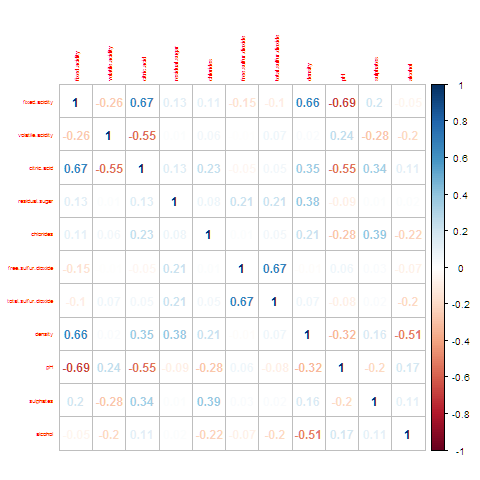
\includegraphics[scale=0.9]{2015-12-03-correlation-matrix of 11 features}
    


    

    

    As the matrix has shown us, it is obvious to see that
total.sulfur.dioxide has linearly correlated with other variables;
therefore, I am not going not include this feature in any classifier.

    \begin{Verbatim}[commandchars=\\\{\}]
{\color{incolor}In [{\color{incolor}6}]:} \PY{c+c1}{\PYZsh{}Remove total.sulfur.dioxide from data.frame}
        wineTrain \PY{o}{\PYZlt{}\PYZhy{}} wineTrain\PY{p}{[} \PY{p}{,} \PY{o}{\PYZhy{}}\PY{k+kp}{which}\PY{p}{(}\PY{k+kp}{names}\PY{p}{(}wineTrain\PY{p}{)} \PY{o}{\PYZpc{}in\PYZpc{}} \PY{k+kt}{c}\PY{p}{(}\PY{l+s}{\PYZdq{}}\PY{l+s}{total.sulfur.dioxide\PYZdq{}}\PY{p}{)}\PY{p}{)}\PY{p}{]}
        wineTest \PY{o}{\PYZlt{}\PYZhy{}} wineTest\PY{p}{[} \PY{p}{,} \PY{o}{\PYZhy{}}\PY{k+kp}{which}\PY{p}{(}\PY{k+kp}{names}\PY{p}{(}wineTest\PY{p}{)} \PY{o}{\PYZpc{}in\PYZpc{}} \PY{k+kt}{c}\PY{p}{(}\PY{l+s}{\PYZdq{}}\PY{l+s}{total.sulfur.dioxide\PYZdq{}}\PY{p}{)}\PY{p}{)}\PY{p}{]}
\end{Verbatim}

    \textbf{d. Normalize data }

In the ``caret'' package, I use the function preProcess to normalize all
the features in the dataset (from the \(1^{st}\) column to the
\(10^{th}\) column ) with the method ``range''

    \begin{Verbatim}[commandchars=\\\{\}]
{\color{incolor}In [{\color{incolor}7}]:} train\PYZus{}normalized \PY{o}{\PYZlt{}\PYZhy{}} preProcess\PY{p}{(}wineTrain\PY{p}{[}\PY{p}{,} \PY{l+m}{1}\PY{o}{:}\PY{l+m}{10}\PY{p}{]}\PY{p}{,} method \PY{o}{=} \PY{l+s}{\PYZsq{}}\PY{l+s}{range\PYZsq{}}\PY{p}{)}
        train\PYZus{}plot \PY{o}{\PYZlt{}\PYZhy{}} predict\PY{p}{(}train\PYZus{}normalized\PY{p}{,} wineTrain\PY{p}{[}\PY{p}{,} \PY{l+m}{1}\PY{o}{:}\PY{l+m}{10}\PY{p}{]}\PY{p}{)}
        png\PY{p}{(}\PY{k+kp}{paste0}\PY{p}{(}today\PY{p}{,} \PY{l+s}{\PYZsq{}}\PY{l+s}{\PYZhy{}\PYZsq{}}\PY{p}{,} \PY{l+s}{\PYZsq{}}\PY{l+s}{feature\PYZhy{}plot.png\PYZsq{}}\PY{p}{)}\PY{p}{)}
        featurePlot\PY{p}{(}train\PYZus{}plot\PY{p}{,} wineTrain\PY{o}{\PYZdl{}}quality\PY{p}{,} \PY{l+s}{\PYZsq{}}\PY{l+s}{box\PYZsq{}}\PY{p}{)}
        dev.off\PY{p}{(}\PY{p}{)}
\end{Verbatim}

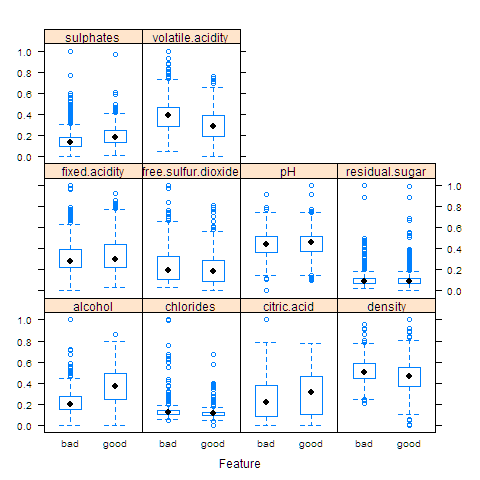
\includegraphics[scale=0.9]{2015-12-03-feature-plot}
    

    From the figure, it looks like alcohol, citric.acid and density separate
most with regard to good classification. Then these 3 features will be
included in Machine Learning models.\hfill \break

\textbf{e. Resampling data}

The function trainControl in the caret package is a very comfortable way
to set the resampling data we need. Among the resampling methods which
accepts as argument, there are an extensive of choices such as
bootstrap, cross validation, and repeated cross validation\ldots{} In
this project, I would like to demonstrate the resampling data's process
by using cross validation method with the number of folds is 10.

    \begin{Verbatim}[commandchars=\\\{\}]
{\color{incolor}In [{\color{incolor}8}]:} fitControl \PY{o}{\PYZlt{}\PYZhy{}} trainControl\PY{p}{(}method \PY{o}{=} \PY{l+s}{\PYZsq{}}\PY{l+s}{cv\PYZsq{}}\PY{p}{,} number \PY{o}{=} \PY{l+m}{10}\PY{p}{)}
\end{Verbatim}

    \textbf{4. Model Selection}

In this section, I would like to apply 3 supervised learning models
which I researched. There are Naive Bayes, K-Nearest Neighbor and Random
Forests. Through every models, I present the way how we input parameters
of the train data into a model in ``caret'' library. Then, the next step
is predicting on the test dataset, which based on the result of train
data. Afterall, the confusion matrix is constructed to compute the
accuracy of the chosen model. Furthermore, I discover that ``caret''
library has provided us a function to calculate the level of importance
of the attributes; therefore, I also include this function in the script
and visualize it for better evaluation what important features of the
model.

\textbf{a. Naive Bayes}

    \begin{Verbatim}[commandchars=\\\{\}]
{\color{incolor}In [{\color{incolor}9}]:} \PY{c+c1}{\PYZsh{}\PYZsh{}\PYZsh{}\PYZsh{}\PYZsh{}\PYZsh{}\PYZsh{}\PYZsh{}\PYZsh{}\PYZsh{}\PYZsh{}\PYZsh{}\PYZsh{}\PYZsh{}\PYZsh{}\PYZsh{}\PYZsh{}\PYZsh{}\PYZsh{}\PYZsh{}\PYZsh{}\PYZsh{}\PYZsh{}\PYZsh{}\PYZsh{}\PYZsh{}\PYZsh{}\PYZsh{}\PYZsh{}\PYZsh{}\PYZsh{}\PYZsh{}\PYZsh{}\PYZsh{}\PYZsh{}\PYZsh{}\PYZsh{}\PYZsh{}\PYZsh{}\PYZsh{}\PYZsh{}\PYZsh{}\PYZsh{}\PYZsh{}\PYZsh{}\PYZsh{}}
        \PY{c+c1}{\PYZsh{}\PYZsh{}\PYZsh{}\PYZsh{}\PYZsh{}\PYZsh{}\PYZsh{}\PYZsh{}\PYZsh{}\PYZsh{}\PYZsh{}\PYZsh{}\PYZsh{}\PYZsh{}\PYZsh{}NAIVEBAYES\PYZsh{}\PYZsh{}\PYZsh{}\PYZsh{}\PYZsh{}\PYZsh{}\PYZsh{}\PYZsh{}\PYZsh{}\PYZsh{}\PYZsh{}\PYZsh{}\PYZsh{}\PYZsh{}\PYZsh{}\PYZsh{}\PYZsh{}\PYZsh{}\PYZsh{}\PYZsh{}\PYZsh{}}
        \PY{c+c1}{\PYZsh{}\PYZsh{}\PYZsh{}\PYZsh{}\PYZsh{}\PYZsh{}\PYZsh{}\PYZsh{}\PYZsh{}\PYZsh{}\PYZsh{}\PYZsh{}\PYZsh{}\PYZsh{}\PYZsh{}\PYZsh{}\PYZsh{}\PYZsh{}\PYZsh{}\PYZsh{}\PYZsh{}\PYZsh{}\PYZsh{}\PYZsh{}\PYZsh{}\PYZsh{}\PYZsh{}\PYZsh{}\PYZsh{}\PYZsh{}\PYZsh{}\PYZsh{}\PYZsh{}\PYZsh{}\PYZsh{}\PYZsh{}\PYZsh{}\PYZsh{}\PYZsh{}\PYZsh{}\PYZsh{}\PYZsh{}\PYZsh{}\PYZsh{}\PYZsh{}\PYZsh{}}
        fit\PYZus{}nb \PY{o}{\PYZlt{}\PYZhy{}} train\PY{p}{(}x \PY{o}{=} wineTrain\PY{p}{[}\PY{p}{,} \PY{l+m}{1}\PY{o}{:}\PY{l+m}{10}\PY{p}{]}\PY{p}{,} y \PY{o}{=} wineTrain\PY{o}{\PYZdl{}}quality\PY{p}{,}
                        method \PY{o}{=}\PY{l+s}{\PYZsq{}}\PY{l+s}{nb\PYZsq{}}\PY{p}{,}trControl \PY{o}{=} fitControl\PY{p}{)}
        predict\PYZus{}nb \PY{o}{\PYZlt{}\PYZhy{}} predict\PY{p}{(}fit\PYZus{}nb\PY{p}{,} newdata \PY{o}{=} wineTest\PY{p}{[}\PY{p}{,} \PY{l+m}{1}\PY{o}{:}\PY{l+m}{10}\PY{p}{]}\PY{p}{)}
        confMat\PYZus{}nb \PY{o}{\PYZlt{}\PYZhy{}} confusionMatrix\PY{p}{(}predict\PYZus{}nb\PY{p}{,} wineTest\PY{o}{\PYZdl{}}quality\PY{p}{,} positive \PY{o}{=} \PY{l+s}{\PYZsq{}}\PY{l+s}{good\PYZsq{}}\PY{p}{)}
        importance\PYZus{}nb \PY{o}{\PYZlt{}\PYZhy{}} varImp\PY{p}{(}fit\PYZus{}nb\PY{p}{,} scale \PY{o}{=} \PY{k+kc}{TRUE}\PY{p}{)}
        
        confMat\PYZus{}nb
        
        png\PY{p}{(}\PY{k+kp}{paste0}\PY{p}{(}today\PY{p}{,} \PY{l+s}{\PYZsq{}}\PY{l+s}{\PYZhy{}\PYZsq{}}\PY{p}{,} \PY{l+s}{\PYZsq{}}\PY{l+s}{importance\PYZhy{}nb.png\PYZsq{}}\PY{p}{)}\PY{p}{)}
        plot\PY{p}{(}importance\PYZus{}nb\PY{p}{,} main \PY{o}{=} \PY{l+s}{\PYZsq{}}\PY{l+s}{Feature importance for Naive Bayes\PYZsq{}}\PY{p}{)}
        dev.off\PY{p}{(}\PY{p}{)}
\end{Verbatim}


            \begin{Verbatim}[commandchars=\\\{\}]
{\color{outcolor}Out[{\color{outcolor}9}]:} Confusion Matrix and Statistics
        
                  Reference
        Prediction bad good
              bad  171   75
              good  52  181
                                                  
                       Accuracy : 0.7349          
                         95\% CI : (0.6929, 0.7739)
            No Information Rate : 0.5344          
            P-Value [Acc > NIR] : < 2e-16         
                                                  
                          Kappa : 0.4707          
         Mcnemar's Test P-Value : 0.05092         
                                                  
                    Sensitivity : 0.7070          
                    Specificity : 0.7668          
                 Pos Pred Value : 0.7768          
                 Neg Pred Value : 0.6951          
                     Prevalence : 0.5344          
                 Detection Rate : 0.3779          
           Detection Prevalence : 0.4864          
              Balanced Accuracy : 0.7369          
                                                  
               'Positive' Class : good            
                                                  
\end{Verbatim}

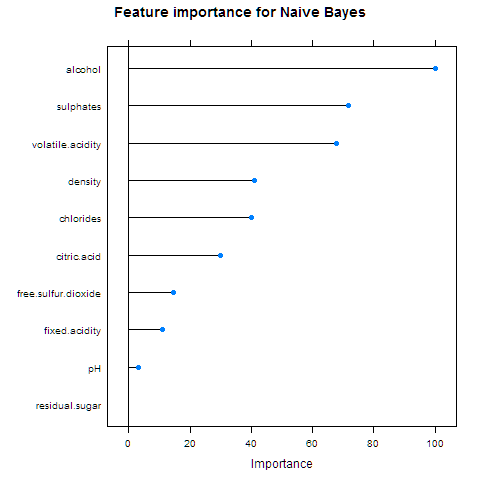
\includegraphics[scale=0.9]{2015-12-03-importance-nb}

    

    

    \textbf{b. K-Nearest Neighbor }

    \begin{Verbatim}[commandchars=\\\{\}]
{\color{incolor}In [{\color{incolor}10}]:} \PY{c+c1}{\PYZsh{}\PYZsh{}\PYZsh{}\PYZsh{}\PYZsh{}\PYZsh{}\PYZsh{}\PYZsh{}\PYZsh{}\PYZsh{}\PYZsh{}\PYZsh{}\PYZsh{}\PYZsh{}\PYZsh{}\PYZsh{}\PYZsh{}\PYZsh{}\PYZsh{}\PYZsh{}\PYZsh{}\PYZsh{}\PYZsh{}\PYZsh{}\PYZsh{}\PYZsh{}\PYZsh{}\PYZsh{}\PYZsh{}\PYZsh{}\PYZsh{}\PYZsh{}\PYZsh{}\PYZsh{}\PYZsh{}\PYZsh{}\PYZsh{}\PYZsh{}\PYZsh{}\PYZsh{}\PYZsh{}\PYZsh{}\PYZsh{}\PYZsh{}\PYZsh{}\PYZsh{}}
         \PY{c+c1}{\PYZsh{}\PYZsh{}\PYZsh{}\PYZsh{}\PYZsh{}\PYZsh{}\PYZsh{}\PYZsh{}\PYZsh{}\PYZsh{}\PYZsh{}\PYZsh{}\PYZsh{}\PYZsh{}\PYZsh{}\PYZsh{}\PYZsh{}\PYZsh{}\PYZsh{}\PYZsh{}\PYZsh{}KNN\PYZsh{}\PYZsh{}\PYZsh{}\PYZsh{}\PYZsh{}\PYZsh{}\PYZsh{}\PYZsh{}\PYZsh{}\PYZsh{}\PYZsh{}\PYZsh{}\PYZsh{}\PYZsh{}\PYZsh{}\PYZsh{}\PYZsh{}\PYZsh{}\PYZsh{}\PYZsh{}\PYZsh{}\PYZsh{}}
         \PY{c+c1}{\PYZsh{}\PYZsh{}\PYZsh{}\PYZsh{}\PYZsh{}\PYZsh{}\PYZsh{}\PYZsh{}\PYZsh{}\PYZsh{}\PYZsh{}\PYZsh{}\PYZsh{}\PYZsh{}\PYZsh{}\PYZsh{}\PYZsh{}\PYZsh{}\PYZsh{}\PYZsh{}\PYZsh{}\PYZsh{}\PYZsh{}\PYZsh{}\PYZsh{}\PYZsh{}\PYZsh{}\PYZsh{}\PYZsh{}\PYZsh{}\PYZsh{}\PYZsh{}\PYZsh{}\PYZsh{}\PYZsh{}\PYZsh{}\PYZsh{}\PYZsh{}\PYZsh{}\PYZsh{}\PYZsh{}\PYZsh{}\PYZsh{}\PYZsh{}\PYZsh{}\PYZsh{}}
         fit\PYZus{}knn \PY{o}{\PYZlt{}\PYZhy{}} train\PY{p}{(}x \PY{o}{=} wineTrain\PY{p}{[}\PY{p}{,} \PY{l+m}{1}\PY{o}{:}\PY{l+m}{10}\PY{p}{]}\PY{p}{,} y \PY{o}{=} wineTrain\PY{o}{\PYZdl{}}quality\PY{p}{,}
                          method \PY{o}{=} \PY{l+s}{\PYZsq{}}\PY{l+s}{knn\PYZsq{}}\PY{p}{,}
                          preProcess \PY{o}{=} \PY{l+s}{\PYZsq{}}\PY{l+s}{range\PYZsq{}}\PY{p}{,} 
                          trControl \PY{o}{=} fitControl\PY{p}{,} 
                          tuneGrid \PY{o}{=} \PY{k+kp}{expand.grid}\PY{p}{(}\PY{l+m}{.}k \PY{o}{=} 
                                   \PY{k+kt}{c}\PY{p}{(}\PY{l+m}{3}\PY{p}{,} \PY{l+m}{5}\PY{p}{,} \PY{l+m}{7}\PY{p}{,} \PY{l+m}{9}\PY{p}{,} \PY{l+m}{11}\PY{p}{,} \PY{l+m}{15}\PY{p}{,} \PY{l+m}{21}\PY{p}{,} \PY{l+m}{25}\PY{p}{,} \PY{l+m}{31}\PY{p}{,} \PY{l+m}{41}\PY{p}{,} \PY{l+m}{51}\PY{p}{,} \PY{l+m}{75}\PY{p}{,} \PY{l+m}{101}\PY{p}{)}\PY{p}{)}\PY{p}{)}  
         predict\PYZus{}knn \PY{o}{\PYZlt{}\PYZhy{}} predict\PY{p}{(}fit\PYZus{}knn\PY{p}{,} newdata \PY{o}{=} wineTest\PY{p}{[}\PY{p}{,} \PY{l+m}{1}\PY{o}{:}\PY{l+m}{10}\PY{p}{]}\PY{p}{)}
         confMat\PYZus{}knn \PY{o}{\PYZlt{}\PYZhy{}} confusionMatrix\PY{p}{(}predict\PYZus{}knn\PY{p}{,} wineTest\PY{o}{\PYZdl{}}quality\PY{p}{,} positive \PY{o}{=} \PY{l+s}{\PYZsq{}}\PY{l+s}{good\PYZsq{}}\PY{p}{)}
         confMat\PYZus{}knn
         
         importance\PYZus{}knn \PY{o}{\PYZlt{}\PYZhy{}} varImp\PY{p}{(}fit\PYZus{}knn\PY{p}{,} scale \PY{o}{=} \PY{k+kc}{TRUE}\PY{p}{)}
         
         png\PY{p}{(}\PY{k+kp}{paste0}\PY{p}{(}today\PY{p}{,} \PY{l+s}{\PYZsq{}}\PY{l+s}{\PYZhy{}\PYZsq{}}\PY{p}{,} \PY{l+s}{\PYZsq{}}\PY{l+s}{importance\PYZhy{}knn.png\PYZsq{}}\PY{p}{)}\PY{p}{)}
         plot\PY{p}{(}importance\PYZus{}knn\PY{p}{,} main \PY{o}{=} \PY{l+s}{\PYZsq{}}\PY{l+s}{Feature importance for K\PYZhy{}nearest neighbor\PYZsq{}}\PY{p}{)}
         dev.off\PY{p}{(}\PY{p}{)}
\end{Verbatim}

            \begin{Verbatim}[commandchars=\\\{\}]
{\color{outcolor}Out[{\color{outcolor}10}]:} Confusion Matrix and Statistics
         
                   Reference
         Prediction bad good
               bad  158   71
               good  65  185
                                                   
                        Accuracy : 0.7161          
                          95\% CI : (0.6734, 0.7561)
             No Information Rate : 0.5344          
             P-Value [Acc > NIR] : 3.124e-16       
                                                   
                           Kappa : 0.4304          
          Mcnemar's Test P-Value : 0.6681          
                                                   
                     Sensitivity : 0.7227          
                     Specificity : 0.7085          
                  Pos Pred Value : 0.7400          
                  Neg Pred Value : 0.6900          
                      Prevalence : 0.5344          
                  Detection Rate : 0.3862          
            Detection Prevalence : 0.5219          
               Balanced Accuracy : 0.7156          
                                                   
                'Positive' Class : good            
                                                   
\end{Verbatim}

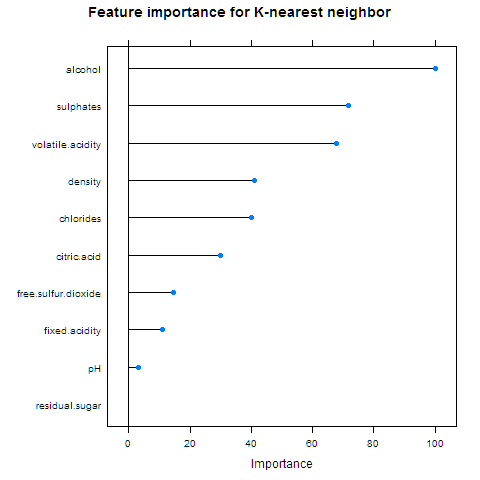
\includegraphics[scale=0.9]{2015-12-03-importance-knn}
    

    

    \textbf{c. Random Forests }

    \begin{Verbatim}[commandchars=\\\{\}]
{\color{incolor}In [{\color{incolor}11}]:} \PY{c+c1}{\PYZsh{}\PYZsh{}\PYZsh{}\PYZsh{}\PYZsh{}\PYZsh{}\PYZsh{}\PYZsh{}\PYZsh{}\PYZsh{}\PYZsh{}\PYZsh{}\PYZsh{}\PYZsh{}\PYZsh{}\PYZsh{}\PYZsh{}\PYZsh{}\PYZsh{}\PYZsh{}\PYZsh{}\PYZsh{}\PYZsh{}\PYZsh{}\PYZsh{}\PYZsh{}\PYZsh{}\PYZsh{}\PYZsh{}\PYZsh{}\PYZsh{}\PYZsh{}\PYZsh{}\PYZsh{}\PYZsh{}\PYZsh{}\PYZsh{}\PYZsh{}\PYZsh{}\PYZsh{}\PYZsh{}\PYZsh{}\PYZsh{}\PYZsh{}\PYZsh{}\PYZsh{}}
         \PY{c+c1}{\PYZsh{}\PYZsh{}\PYZsh{}\PYZsh{}\PYZsh{}\PYZsh{}\PYZsh{}\PYZsh{}\PYZsh{}\PYZsh{}\PYZsh{}\PYZsh{}\PYZsh{}RANDOMFORESTS\PYZsh{}\PYZsh{}\PYZsh{}\PYZsh{}\PYZsh{}\PYZsh{}\PYZsh{}\PYZsh{}\PYZsh{}\PYZsh{}\PYZsh{}\PYZsh{}\PYZsh{}\PYZsh{}\PYZsh{}\PYZsh{}\PYZsh{}\PYZsh{}\PYZsh{}\PYZsh{}}
         \PY{c+c1}{\PYZsh{}\PYZsh{}\PYZsh{}\PYZsh{}\PYZsh{}\PYZsh{}\PYZsh{}\PYZsh{}\PYZsh{}\PYZsh{}\PYZsh{}\PYZsh{}\PYZsh{}\PYZsh{}\PYZsh{}\PYZsh{}\PYZsh{}\PYZsh{}\PYZsh{}\PYZsh{}\PYZsh{}\PYZsh{}\PYZsh{}\PYZsh{}\PYZsh{}\PYZsh{}\PYZsh{}\PYZsh{}\PYZsh{}\PYZsh{}\PYZsh{}\PYZsh{}\PYZsh{}\PYZsh{}\PYZsh{}\PYZsh{}\PYZsh{}\PYZsh{}\PYZsh{}\PYZsh{}\PYZsh{}\PYZsh{}\PYZsh{}\PYZsh{}\PYZsh{}\PYZsh{}}
         
         fit\PYZus{}rf \PY{o}{\PYZlt{}\PYZhy{}} train\PY{p}{(}x \PY{o}{=} wineTrain\PY{p}{[}\PY{p}{,} \PY{l+m}{1}\PY{o}{:}\PY{l+m}{10}\PY{p}{]}\PY{p}{,} y \PY{o}{=} wineTrain\PY{o}{\PYZdl{}}quality\PY{p}{,}
                         method \PY{o}{=} \PY{l+s}{\PYZsq{}}\PY{l+s}{rf\PYZsq{}}\PY{p}{,}
                         trControl \PY{o}{=} fitControl\PY{p}{,}
                         tuneGrid \PY{o}{=} \PY{k+kp}{expand.grid}\PY{p}{(}\PY{l+m}{.}mtry \PY{o}{=} \PY{k+kt}{c}\PY{p}{(}\PY{l+m}{2}\PY{o}{:}\PY{l+m}{6}\PY{p}{)}\PY{p}{)}\PY{p}{,}
                         n.tree \PY{o}{=} \PY{l+m}{500}\PY{p}{)} 
         predict\PYZus{}rf \PY{o}{\PYZlt{}\PYZhy{}} predict\PY{p}{(}fit\PYZus{}rf\PY{p}{,} newdata \PY{o}{=} wineTest\PY{p}{[}\PY{p}{,} \PY{l+m}{1}\PY{o}{:}\PY{l+m}{10}\PY{p}{]}\PY{p}{)}
         confMat\PYZus{}rf \PY{o}{\PYZlt{}\PYZhy{}} confusionMatrix\PY{p}{(}predict\PYZus{}rf\PY{p}{,} wineTest\PY{o}{\PYZdl{}}quality\PY{p}{,} positive \PY{o}{=} \PY{l+s}{\PYZsq{}}\PY{l+s}{good\PYZsq{}}\PY{p}{)}
         
         confMat\PYZus{}rf
         
         importance\PYZus{}rf \PY{o}{\PYZlt{}\PYZhy{}} varImp\PY{p}{(}fit\PYZus{}rf\PY{p}{,} scale \PY{o}{=} \PY{k+kc}{TRUE}\PY{p}{)}
         
         png\PY{p}{(}\PY{k+kp}{paste0}\PY{p}{(}today\PY{p}{,} \PY{l+s}{\PYZsq{}}\PY{l+s}{\PYZhy{}\PYZsq{}}\PY{p}{,} \PY{l+s}{\PYZsq{}}\PY{l+s}{importance\PYZhy{}rf.png\PYZsq{}}\PY{p}{)}\PY{p}{)}
         plot\PY{p}{(}importance\PYZus{}rf\PY{p}{,} main \PY{o}{=} \PY{l+s}{\PYZsq{}}\PY{l+s}{Feature importance for Random Forests\PYZsq{}}\PY{p}{)}
         dev.off\PY{p}{(}\PY{p}{)}
\end{Verbatim}

            \begin{Verbatim}[commandchars=\\\{\}]
{\color{outcolor}Out[{\color{outcolor}11}]:} Confusion Matrix and Statistics
         
                   Reference
         Prediction bad good
               bad  172   49
               good  51  207
                                                  
                        Accuracy : 0.7912         
                          95\% CI : (0.752, 0.8268)
             No Information Rate : 0.5344         
             P-Value [Acc > NIR] : <2e-16         
                                                  
                           Kappa : 0.5802         
          Mcnemar's Test P-Value : 0.9203         
                                                  
                     Sensitivity : 0.8086         
                     Specificity : 0.7713         
                  Pos Pred Value : 0.8023         
                  Neg Pred Value : 0.7783         
                      Prevalence : 0.5344         
                  Detection Rate : 0.4322         
            Detection Prevalence : 0.5386         
               Balanced Accuracy : 0.7899         
                                                  
                'Positive' Class : good           
                                                  
\end{Verbatim}

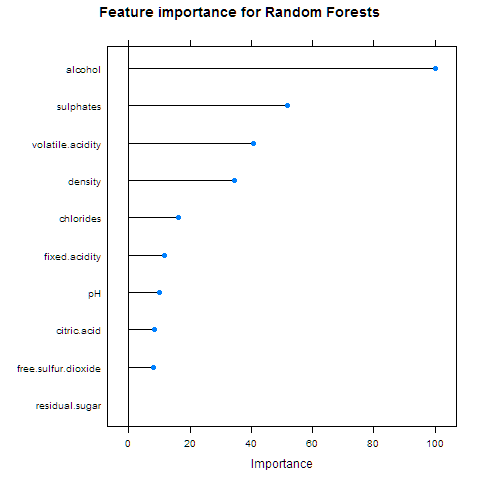
\includegraphics[scale=0.9]{2015-12-03-importance-rf}

    

    

   \textbf{d. Tunning parameters}

Due to the lack of resources, I just try to tunning parameters in Random
Forests. Thus, I choose the number of trees in the algorithm for the
purpose to evaluate what it affect the accuracy of the model.

    \begin{Verbatim}[commandchars=\\\{\}]
{\color{incolor}In [{\color{incolor}12}]:} ntree \PY{o}{\PYZlt{}\PYZhy{}} \PY{k+kt}{c}\PY{p}{(}\PY{l+m}{1}\PY{p}{,} \PY{l+m}{30}\PY{p}{,} \PY{l+m}{50}\PY{p}{,} \PY{l+m}{80}\PY{p}{,} \PY{l+m}{120}\PY{p}{,} \PY{l+m}{150}\PY{p}{,} \PY{l+m}{200}\PY{p}{,} \PY{l+m}{300}\PY{p}{,} \PY{l+m}{500}\PY{p}{,} \PY{l+m}{550}\PY{p}{,} \PY{l+m}{700}\PY{p}{)} \PY{c+c1}{\PYZsh{}Vector number of trees}
\end{Verbatim}

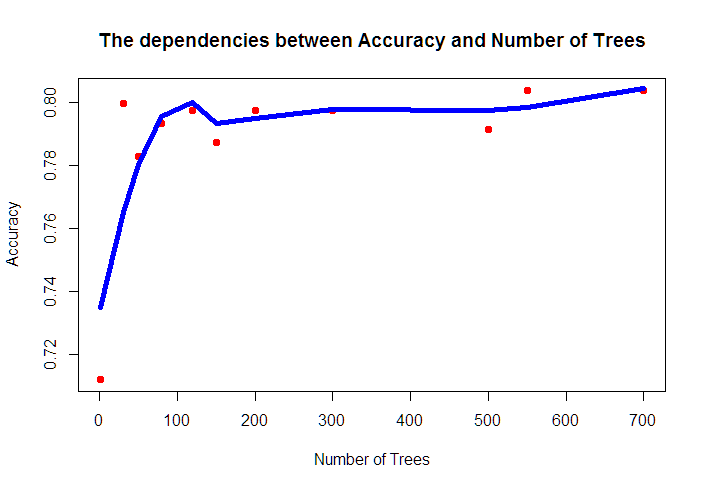
\includegraphics[scale=0.6]{Acc-tree}
    

    \textbf{5. Evaluate the accuracy of the three chosen model}

    \begin{Verbatim}[commandchars=\\\{\}]
{\color{incolor}In [{\color{incolor}13}]:} models \PY{o}{\PYZlt{}\PYZhy{}} resamples\PY{p}{(}\PY{k+kt}{list}\PY{p}{(}NB \PY{o}{=} fit\PYZus{}nb\PY{p}{,} KNN \PY{o}{=} fit\PYZus{}knn\PY{p}{,}
                                  RF \PY{o}{=} fit\PYZus{}rf\PY{p}{)}\PY{p}{)}
         png\PY{p}{(}\PY{k+kp}{paste0}\PY{p}{(}today\PY{p}{,} \PY{l+s}{\PYZsq{}}\PY{l+s}{\PYZhy{}\PYZsq{}}\PY{p}{,} \PY{l+s}{\PYZsq{}}\PY{l+s}{models\PYZhy{}comparison.png\PYZsq{}}\PY{p}{)}\PY{p}{)}
         dotplot\PY{p}{(}models\PY{p}{)}
         dev.off\PY{p}{(}\PY{p}{)}
\end{Verbatim}



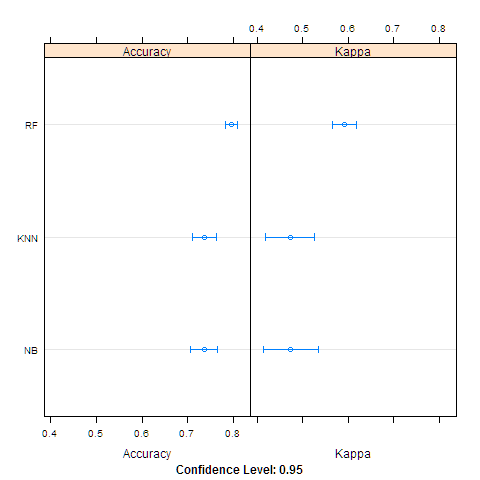
\includegraphics[scale=0.8]{2015-12-03-models-comparison}

    

    \begin{Verbatim}[commandchars=\\\{\}]
{\color{incolor}In [{\color{incolor}14}]:} results \PY{o}{\PYZlt{}\PYZhy{}} \PY{k+kp}{summary}\PY{p}{(}models\PY{p}{)}
         png\PY{p}{(}\PY{k+kp}{paste0}\PY{p}{(}today\PY{p}{,} \PY{l+s}{\PYZsq{}}\PY{l+s}{\PYZhy{}\PYZsq{}}\PY{p}{,} \PY{l+s}{\PYZsq{}}\PY{l+s}{models\PYZhy{}accuracy.png\PYZsq{}}\PY{p}{)}\PY{p}{,} width \PY{o}{=} \PY{l+m}{480}\PY{p}{,} height \PY{o}{=} \PY{l+m}{180}\PY{p}{)}
         grid.table\PY{p}{(}results\PY{o}{\PYZdl{}}statistics\PY{o}{\PYZdl{}}Accuracy\PY{p}{)}
         dev.off\PY{p}{(}\PY{p}{)}
\end{Verbatim}

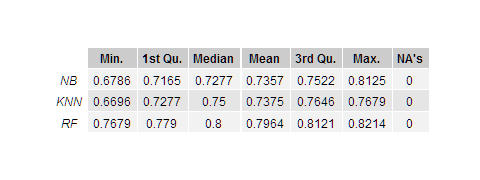
\includegraphics[scale=1]{2015-12-03-models-accuracy}
    

    

    \section*{IV. Conclusion}\label{iv.-conclusion}

\hspace{5mm}It does not look like wine quality is well supported by its chemical
properties ( We can easily see that in feature important of 3 chosen
models). At each quality level variability of the predictors is high and
the groups are not well separated.

The total.sulfur.dioxide is highly correlated and should be excluded
from any classifier.

The acohol attribute strongly affects wines belonged to which class.

Between 3 chosen models, Random Forests gives us the best result.


    % Add a bibliography block to the postdoc
    
    
    
    \end{document}
